\documentclass{prova}

\usepackage{amsmath}
\usepackage{amsfonts}

\setlength{\textheight}{25cm}

\renewcommand{\sin}{\,\mbox{sen}\,}
\DeclareMathOperator{\tg}{tg}
\newcommand{\ds}{\displaystyle}

\professor{Prof.\@ Adriano Barbosa}
\disciplina{Introdu\c{c}\~ao ao C\'alculo}
\avaliacao{Final}
\curso{Qu\'{\i}mica}
\data{12/09/2023}

\begin{document}
	\cabecalho{5}  % o numero 5 indica a qnt de quadros na tabela de nota

    \textbf{Todas as respostas devem ser justificadas.}

    \begin{questionario}
        \q{Dados os intervalos da forma $\ds\left[0, \frac{1}{n}\right]$, com
           $n\in\mathbb{N}$. Pergunta-se:}
            \begin{questionario}
                \qq{Existe algum n\'umero real comum a todos os intervalos?}
                \qq{E se os intervalos fossem abertos,
                    $\ds\left(0,\frac{1}{n}\right)$, com $n\in\mathbb{N}$?}
            \end{questionario}
        \q{Uma sequ\^encia com 2023 hex\'agonos foi montada como na figura abaixo.
           Quantas arestas existem na sequ\^encia?}
           \begin{figure}[h]
               \centering
               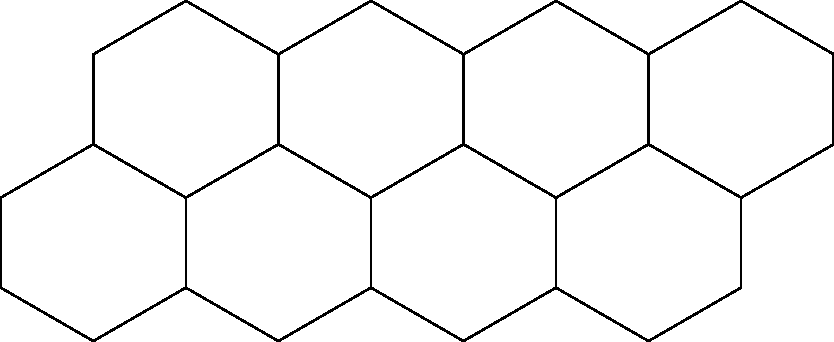
\includegraphics[width=0.5\textwidth]{fig1.pdf}
           \end{figure}
	    \q{Dada a fun\c{c}\~ao quadr\'atica $f:[0,1]\rightarrow\mathbb{R}$,
           $f(x)=x^2-4x+1$, determine seu valor m\'aximo e m\'{\i}nimo e para quais
           valores de $x$ eles s\~ao atingidos.}
        \q{Se o crescimento de uma popula\c{c}\~ao \'e de 20\% ao ano, determine em
           quanto tempo essa popula\c{c}\~ao dobrar\'a de tamanho. (Utilize $\log 2=0,3$ e
           $\log 3=0,48$)}
        \q{Calcule $\sin{x}$ e $\cos{x}$ sabendo que $\tg{x}+\sec{x}=\ds\frac{3}{2}$.}
    \end{questionario}
\end{document}
